
\chapter{Statistics and Probability}
\section{Definition of Moments}
Let $x\in\mathbb R^{n}$ is a random variable.
We write $m = E[x]\in\mathbb R^n$ for the expectation and
$M=\mathrm{Var}[x] = E[(x-m)(x-m)^T]$ for the covariance (when these quantities are defined.)

In tensor diagrams, we will use square brackets:
\[
   \vecmatvec{1em}{}{}{m}
   =
\mathbin{\begin{tikzpicture}[baseline=(n0.base), inner sep=1pt]
   \node (n0) at (0,0) {$[$};
   \node [right=1em of n0] (n1) {$x]$};
   \draw (n0) -- (n1);
\end{tikzpicture}}
\quad\text{and}\quad
   \vecmatvec{1em}{}{M}{}
   =
\mathbin{\begin{tikzpicture}[baseline=(n0.base), inner sep=1pt]
   \node (n0) at (0,0) {$[$};
   \node [right=1em of n0] (n1) {$(x\ominus m)$};
   \node [right=.5em of n1] (n2) {$(x\ominus m)$};
   \node [right=1em of n2] (n3) {$]$};
   \draw (n0) -- (n1);
   \draw (n2) -- (n3);
\end{tikzpicture}}
\]
We will use the circled minus, $\ominus$, to distinguish the operation from contraction edges.

We can also define the third and fourth centralized moment tensors
\[
   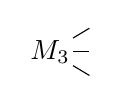
\begin{tikzpicture}[baseline=(T.base), inner sep=1pt]
      \node (T) {$M_3$};
      \draw (T) -- ++(.5,.3);
      \draw (T) -- ++(.5,-.3);
      \draw (T) -- ++(.5,0);
   \end{tikzpicture}
   =
   \renewcommand*{\arraystretch}{1.3}
   \begin{bmatrix}
      \vecmatvec{1em}{(x\ominus m)}{}{} \\
      \vecmatvec{1em}{(x\ominus m)}{}{} \\
      \vecmatvec{1em}{(x\ominus m)}{}{}
   \end{bmatrix}
\quad\text{and}\quad
   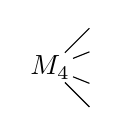
\begin{tikzpicture}[baseline=(T.base), inner sep=1pt]
      \node (T) {$M_4$};
      \draw (T) -- ++(.5,.5);
      \draw (T) -- ++(.5,-.5);
      \draw (T) -- ++(.5,.2);
      \draw (T) -- ++(.5,-.2);
   \end{tikzpicture}
   =
   \renewcommand*{\arraystretch}{1.3}
   \begin{bmatrix}
      \vecmatvec{1em}{(x\ominus m)}{}{} \\
      \vecmatvec{1em}{(x\ominus m)}{}{} \\
      \vecmatvec{1em}{(x\ominus m)}{}{} \\
      \vecmatvec{1em}{(x\ominus m)}{}{}
   \end{bmatrix}
.
\]
%These are less common in introductory causes, even though the scalar third and fourth moment are common.
%This is presumably because they require higher order tensors.

%If the entries of $x$ are independent, the non-diagonal entries disappear, so we get
%\[
%M =
%\left[
%   \begin{tikzpicture}[baseline=(c.base), inner sep=1pt]
%      \node (T1) {$(x\ominus m)$};
%      \node (T2)[below=.5em of T1] {$(x\ominus m)$};
%      \node (c)[right=.7em of T1, yshift=-1em] {$\sbullet$};
%      \draw (T1) -- (c);
%      \draw (T2) -- (c);
%      \draw (c) -- ++(.7em,0);
%   \end{tikzpicture}
%\right]
%\quad\text{and}\quad
%M_3 =
%\left[
%   \begin{tikzpicture}[baseline=(T2.base), inner sep=1pt]
%      \node (T1) {$(x\ominus m)$};
%      \node (T2)[below=.5em of T1] {$(x\ominus m)$};
%      \node (T3)[below=.5em of T2] {$(x\ominus m)$};
%      \node (c)[right=.7em of T2] {$\sbullet$};
%      \draw (T1) -- (c);
%      \draw (T2) -- (c);
%      \draw (T3) -- (c);
%      \draw (c) -- ++(.7em,0);
%   \end{tikzpicture}
%\right]
%\quad\text{and so on.}
%\]
% If the entries are also identically distributed, we simply have
% \[
%    M = \sigma^2
%    \,
% \begin{tikzpicture}[baseline=(T.base), inner sep=0]
%    \node (T) {$\sbullet$};
%    \draw (T) -- ++(0,.3);
%    \draw (T) -- ++(0,-.3);
% \end{tikzpicture}
%    \text{ and }
%    M_3 = \mathrm{E}[(x_0-m_0)^3]
% \begin{tikzpicture}[baseline=(T.base), inner sep=0]
%    \node (T) {$\sbullet$};
%    \draw (T) -- ++(0,.3);
%    \draw (T) -- ++(-.2,-.3);
%    \draw (T) -- ++(.2,-.3);
% \end{tikzpicture}
% .
% \]


\subsection{Expectation of Linear Combinations}
General principle: The ``linearity of expectation'' lets you pull out all parts of the graph not involving $X$.
\[
   \vcenter{\hbox{
      \import{figures/}{linearityOfExpectation.pdf_tex}
   }}
\]
where $M_3$ is the expectation\footnote{FIXME: This is different from the notation just introduced above.}
\(
\left[
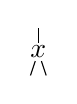
\begin{tikzpicture}[baseline=(T.base), inner sep=1pt]
   \node (T) {$x$};
   \draw (T) -- ++(0,.3);
   \draw (T) -- ++(-.1,-.3);
   \draw (T) -- ++(.1,-.3);
\end{tikzpicture}
\,
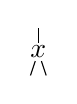
\begin{tikzpicture}[baseline=(T.base), inner sep=1pt]
   \node (T) {$x$};
   \draw (T) -- ++(0,.3);
   \draw (T) -- ++(-.1,-.3);
   \draw (T) -- ++(.1,-.3);
\end{tikzpicture}
\,
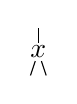
\begin{tikzpicture}[baseline=(T.base), inner sep=1pt]
   \node (T) {$x$};
   \draw (T) -- ++(0,.3);
   \draw (T) -- ++(-.1,-.3);
   \draw (T) -- ++(.1,-.3);
\end{tikzpicture}
\right]
\),
which is an order-9 tensor with no dependence on the constants $A$, $B$, $C$ and $D$.
In practice you would want to name the edges to keep track of what gets multiplied with what.

We can even use linearity of expectation to push the expectation inside an infinite sum of tensors, as in the following moment generating function, which relates all the $M_k$ tensors:
\begin{align*}
   \mathrm{E}(\mathrm{e}^{\langle x\ominus m, t\rangle})
   &= \sum_{k=0}^\infty \frac{1}{k!} \mathrm{E}[\langle x\ominus m, t\rangle^k]
    = \mathrm{E}\big[\sum_{k=0}^\infty \frac{1}{k!} \langle (x\ominus m)^{\otimes k}, t^{\otimes k}\rangle\big]
   = \sum_{k=0}^\infty \frac{1}{k!} \langle M_k, t^{\otimes k}\rangle
 \\&=
  % =
   1
   +
   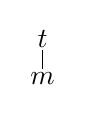
\begin{tikzpicture}[baseline=.5em, inner sep=1]
      \node (T) {$m$};
      \draw (T) -- ++(0,.5) node[fill=white] {$t$};
   \end{tikzpicture}
   +
   \frac{1}{2}
   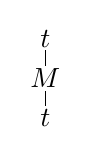
\begin{tikzpicture}[baseline=(T.base), inner sep=1]
      \node (T) {$M$};
      \draw (T) -- ++(0,.5) node[fill=white] {$t$};
      \draw (T) -- ++(0,-.5) node[fill=white] {$t$};
   \end{tikzpicture}
   +
   \frac{1}{6}
   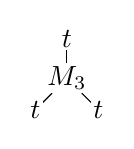
\begin{tikzpicture}[baseline=(T.base), inner sep=1]
      \node (T) {$M_3$};
      \draw (T) -- ++(0,.5) node[fill=white] {$t$};
      \draw (T) -- ++(-.4,-.4) node[fill=white] {$t$};
      \draw (T) -- ++(.4,-.4) node[fill=white] {$t$};
   \end{tikzpicture}
   +
   \frac{1}{24}
   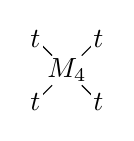
\begin{tikzpicture}[baseline=(T.base), inner sep=1]
      \node (T) {$M_4$};
      \draw (T) -- ++(-.4,-.4) node[fill=white] {$t$};
      \draw (T) -- ++(.4,-.4) node[fill=white] {$t$};
      \draw (T) -- ++(-.4,.4) node[fill=white] {$t$};
      \draw (T) -- ++(.4,.4) node[fill=white] {$t$};
   \end{tikzpicture}
   +
   \dots
\end{align*}

\subsection{Linear Forms}
The Matrix Cookbook gives the following simple expectation:
\begin{walign}
   \tag{312}
   \E[AXB+C] &= A \E[X] B + C
   &
   \renewcommand*{\arraystretch}{1.3}
   \begin{bmatrix}
      \matmul{A,X,B} \\+\, \matmul{C}
   \end{bmatrix}
   &=
   \renewcommand*{\arraystretch}{1.3}
   \begin{matrix}
      \matmul{A,[X],B} \\+\, \matmul{C}
   \end{matrix}
\end{walign}

\subsection{Quadratic Forms}
We often prefer to write expectations in terms of the simple centered moments, which we can do by pulling out the mean:
\renewcommand*{\arraystretch}{1}
\[
   \begin{bmatrix}
      x - \\
      x -
   \end{bmatrix}
   =
   \begin{bmatrix}
      (x\ominus m) - \\
      (x\ominus m) -
   \end{bmatrix}
   +
   \begin{array}{c}
      m - \\
      m -
   \end{array}
   =
   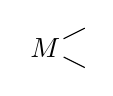
\begin{tikzpicture}[baseline=(T.base), inner sep=1pt]
      \node (T) {$M$};
      \draw (T) -- ++(.5,.25);
      \draw (T) -- ++(.5,-.25);
   \end{tikzpicture}
   +
   \begin{array}{c}
      m - \\
      m -
   \end{array}
\]
This makes it easy to handle the quadratic forms from the Matrix Cookbook:
\begin{walign}
   \tag{313}
   \mathrm{Var}[Ax] &= A \mathrm{Var}[x] A^T
   &
   \renewcommand*{\arraystretch}{1.3}
   \begin{bmatrix}
      \vecmatvec{.5em}{A}{}{x} \ominus [\vecmatvec{.5em}{A}{}{x}] \\
      \vecmatvec{.5em}{A}{}{x} \ominus [\vecmatvec{.5em}{A}{}{x}]
   \end{bmatrix}
   &=
   \renewcommand*{\arraystretch}{1.3}
   \begin{bmatrix}
      \vecmatvec{.5em}{A}{}{(x\ominus m)} \\
      \vecmatvec{.5em}{A}{}{(x\ominus m)}
   \end{bmatrix}
 \\&&&=
   \vcenter{\hbox{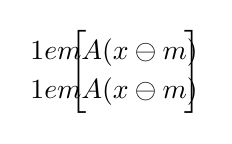
\begin{tikzpicture}[inner sep=1pt]
      \node (n1) at (0,-.25) {$\vecmatvec{1em}{A}{}{(x\ominus m)}$};
      \node (n2) at (0,.25) {$\vecmatvec{1em}{A}{}{(x\ominus m)}$};
      \node at (-.45, 0) {$\Bigg[$};
      \node at (1, 0) {$\Bigg]$};
   \end{tikzpicture}}}
 \\&&& =
   \vecmatvec{.5em}{}{A,M_2,A}{}
%%%%%%%%%%%%%%%%%%%%%%%%%%%%%%%%%%%%%%%%%%%%%%%%%%%%%%%%%%%%%%%%%%%%%%%%%%%%%%%%
   \\[.5em]
   \tag{318}
   \E[x^T A x]
   &= \mathrm{Tr}(A M) + m^T A m
   &
   [\vecmatvec{.5em}{x}{A}{x}]
   &=
   \left(
      \begin{bmatrix}
         (x\ominus m) - \\
         (x\ominus m) -
      \end{bmatrix}
      +
      \begin{array}{c}
         m - \\
         m -
      \end{array}
   \right)
   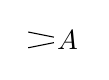
\begin{tikzpicture}[baseline=(A.base), inner sep=1pt]
      \node (A) {$A$};
      \draw (A) -- ++(-.5, .1);
      \draw (A) -- ++(-.5, -.1);
   \end{tikzpicture}
   \\
   &&&=
   \mathbin{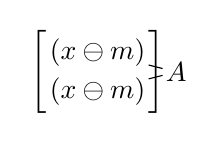
\begin{tikzpicture}[baseline=(A.base), inner sep=1pt]
      \node (n1) at (0,-.25) {$(x\ominus m)$};
      \node (n2) at (0,.25) {$(x\ominus m)$};
      \node at (-.75, 0) {$\Bigg[$};
      \node at (.75, 0) {$\Bigg]$};
      \node (A) at (1, 0) {$A$};
      \draw (n1) -- (A);
      \draw (n2) -- (A);
   \end{tikzpicture}}
   +
   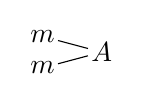
\begin{tikzpicture}[baseline=(A.base), inner sep=1pt]
      \node (A) {$A$};
      \node (m1) at (-.75, .2) {$m$};
      \node (m2) at (-.75, -.2) {$m$};
      \draw (m1) -- (A) -- (m2);
   \end{tikzpicture}
   \\
   &&&=
   \trace{M,A}2
   +
   \vecmatvec{.5em}{m}{A}{m}
   \\[.5em]
\end{walign}

\begin{align*}
   E[(A\mathbf{x} + a)(B\mathbf{x} + b)^T] &= AMB^T + (Am + a)(Bm + b)^T \tag{320} \\
   E[\mathbf{x}\mathbf{x}^T] &= M + mm^T \tag{321} \\
   E[\mathbf{x} a^T \mathbf{x}] &= (M + mm^T)a \tag{322} \\
   E[\mathbf{x}^T a\mathbf{x}^T] &= a^T(M + mm^T) \tag{323} \\
   E[(A\mathbf{x})(A\mathbf{x})^T] &= A(M + mm^T)A^T \tag{324} \\
   E[(\mathbf{x} + a)(\mathbf{x} + a)^T] &= M + (m + a)(m + a)^T \tag{325} \\
   E[(A\mathbf{x} + a)^T(B\mathbf{x} + b)] &= \text{Tr}(AMB^T) + (Am + a)^T(Bm + b) \tag{326} \\
   E[\mathbf{x}^T \mathbf{x}] &= \text{Tr}(M) + m^T m \tag{327} \\
   E[\mathbf{x}^T A\mathbf{x}] &= \text{Tr}(AM) + m^T Am \tag{328} \\
   E[(A\mathbf{x})^T(A\mathbf{x})] &= \text{Tr}(AMA^T) + (Am)^T(Am) \tag{329} \\
   E[(\mathbf{x} + a)^T(\mathbf{x} + a)] &= \text{Tr}(M) + (m + a)^T(m + a) \tag{330}
\end{align*}



\subsection{Cubic Forms}

\[
\begin{tikzpicture}[scale=1.3,
  every node/.style={inner sep=1pt, circle, draw, fill=white, thin},
  label/.style={draw=none, fill=none, text=black, font=\scriptsize},
  declare function={
    xgap=.8;  % Horizontal spacing between diagrams
  }]

  \drawPartitionAtAngle{(-1.6*xgap,0)}{3}{$\kappa_3$}{{{1,2,3}}}
  \drawPartitionAtAngle{(0,0)}{3}{$+\kappa_2\kappa_1\Big($}{{{1,2},{3}}}
  \drawPartitionAtAngle{(xgap,0)}{3}{$+$}{{{1,3},{2}}}
  \drawPartitionAtAngle{(2*xgap,0)}{3}{$+$}{{{2,3},{1}}}
  \drawPartitionAtAngle{(3.6*xgap,0)}{3}{$\Big)+\kappa_1^3$}{{{1},{2},{3}}}

\end{tikzpicture}
\]


When $x$ is a stochastic vector with mean vector $m$,
it can be convenient to expand the raw third moment in terms of the central moments:

\renewcommand*{\arraystretch}{1}
\begin{align*}
\begin{bmatrix}
   x - \\
   x - \\
   x -
\end{bmatrix}
&=
\begin{bmatrix}
   (x\ominus m) - \\
   (x\ominus m) - \\
   (x\ominus m) -
\end{bmatrix}
\vspace{-.5em}
+
3
\hspace{-.25em}
\begin{array}{l}
\begin{bmatrix}
   (x\ominus m) -
\end{bmatrix}\\[.1em]
\begin{bmatrix}
   m - \\
   m -
\end{bmatrix}
\end{array}
\hspace{-.5em}
+
3
\hspace{-.25em}
\begin{array}{l}
\begin{bmatrix}
   m -
\end{bmatrix}\\[.1em]
\begin{bmatrix}
   (x\ominus m) - \\
   (x\ominus m) -
\end{bmatrix}
\end{array}
\hspace{-.5em}
+
\hspace{-.5em}
\begin{array}{c}
\begin{bmatrix}
   m -
\end{bmatrix}\\[.1em]
\begin{bmatrix}
   m -
\end{bmatrix}\\[.1em]
\begin{bmatrix}
   m -
\end{bmatrix}
\end{array}
%
\\&=
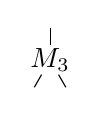
\begin{tikzpicture}[baseline=(T.base), inner sep=1pt]
   \node (T) {$M_3$};
   \draw (T) -- ++(0,.4);
   \draw (T) -- ++(-.2,-.35);
   \draw (T) -- ++(.2,-.35);
\end{tikzpicture}
+
3
\hspace{-.25em}
\begin{array}{c}
   m - \\
   -M-
\end{array}
\hspace{-.5em}
+
\begin{array}{c}
   m - \\
   m - \\
   m -
\end{array}
\end{align*}
TODO: The edges from the $m,M$ term needs to be symmetrized.


But this is still a bit of a mess.
See also below on Cumulants.



Assume \(\mathbf{x}\) to be a stochastic vector with independent coordinates, mean \(m\),
covariance \(M\) and central moments \(v_3 = \mathbb{E}[(\mathbf{x} - m)^3]\). Then (see [7])
\begin{align*}
&\mathbb{E}[(A\mathbf{x} + a)(B\mathbf{x} + b)^T (C\mathbf{x} + c)]
\\&\quad=
A\,\mathrm{diag}(B^T C) v_3
\\&\quad+
(Am + a) \mathrm{Tr}(BMC^T)
\\&\quad+
AMC^T (Bm + b)
\\&\quad\,+
AMB^T (Cm + c)
\\&\quad+
(Am + a)(Bm + b)^T (Cm + c)
\\
  &\mathbb{E}[\mathbf{x} \mathbf{x}^T \mathbf{x}]
\\&\quad=
   v_3
\\&\quad+
   2 Mm
\\&\quad+
   (\text{Tr}(M) + m^T m) m
\end{align*}


\section{Cumulants}

Given a random vector $x\in\mathbb R^d$,
its $n$th Cumulant Tensor, $K_n\in\R^{d,\ldots,d}$ is defined by
\[
   \log \mathrm{E}(\mathrm{e}^{\langle t, x\rangle})
   = \sum_{n=1}^\infty \frac{1}{n!} \langle K_n, t^{\otimes n}\rangle
   =
   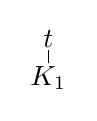
\begin{tikzpicture}[baseline=.5em, inner sep=1]
      \node (T) {$K_1$};
      \draw (T) -- ++(0,.5) node[fill=white] {$t$};
   \end{tikzpicture}
   +
   \frac{1}{2}
   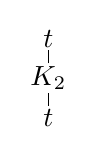
\begin{tikzpicture}[baseline=(T.base), inner sep=1]
      \node (T) {$K_2$};
      \draw (T) -- ++(0,.5) node[fill=white] {$t$};
      \draw (T) -- ++(0,-.5) node[fill=white] {$t$};
   \end{tikzpicture}
   +
   \frac{1}{6}
   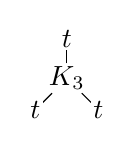
\begin{tikzpicture}[baseline=(T.base), inner sep=1]
      \node (T) {$K_3$};
      \draw (T) -- ++(0,.5) node[fill=white] {$t$};
      \draw (T) -- ++(-.4,-.4) node[fill=white] {$t$};
      \draw (T) -- ++(.4,-.4) node[fill=white] {$t$};
   \end{tikzpicture}
   +
   \dots
\]
The first couple of cumulants are similar to the central moments:
\[
   K_1 = m
   \quad\text{and}\quad
   K_2 = M
   \quad\text{and}\quad
   K_3 = M_3
   \quad\text{and}\quad
   K_4 = M_4
   - \begin{tikzpicture}[baseline=-.8em, inner sep=.5pt]
      \node (M1) {\scriptsize $M_2$};
      \node[below=.4em of M1] (M2) {\scriptsize $M_2$};
      \draw (M1) -- ++(.35,0);
      \draw (M2) -- ++(.35,0);
      \draw (M1) -- ++(-.35,0);
      \draw (M2) -- ++(-.35,0);
   \end{tikzpicture}
   - \begin{tikzpicture}[baseline=(M1.base), inner sep=.5pt]
      \node (M1) {\scriptsize $M_2$};
      \node[right=.05em of M1] (M2) {\scriptsize $M_2$};
      \draw (M1) -- ++(-.25,.25);
      \draw (M1) -- ++(-.25,-.25);
      \draw (M2) -- ++(.25,.25);
      \draw (M2) -- ++(.25,-.25);
   \end{tikzpicture}
   - \begin{tikzpicture}[baseline=(M1.base), inner sep=.5pt]
      \node (M1) {\scriptsize $M_2$};
      \node[right=.05em of M1, yshift=-2pt] (M2) {\scriptsize $M_2$};
      \draw (M1) -- ++(-.25,.25);
      \draw (M1) -- ++(+.7,-.25);
      \draw (M2) -- ++(-.7,-.25);
      \draw (M2) -- ++(.25,.25);
   \end{tikzpicture}
   .
\]
They have the nice property (which is easy to see from the definition) that they are additive for independent random variables:
$
   K_n(x + y) = K_n(x) + K_n(y).
$
This generalizes the standard property that the variance of the sum of independent random variables is the sum of the variances.

We can write the expectations of $x^{\otimes n}$ in terms of the cumulants:

\[
   \begin{bmatrix}
      \begin{tikzpicture}[
         baseline=(T.base),
         every node/.style={inner sep=1pt, circle, draw=none, fill=white},
       ]
       \draw (30:.2) node[label] {$x$} -- (30:.6);
       \draw (150:.2) node[label] {$x$} -- (150:.6);
       \draw (270:.2) node[label] {$x$} -- (270:.6);
      \end{tikzpicture}
   \end{bmatrix}
   =
   \begin{tikzpicture}[
      baseline=-1em,
     every node/.style={inner sep=1pt, circle, draw, fill=white, thin},
     label/.style={draw=none, fill=none, text=black, font=\scriptsize},
     declare function={
       xgap=1.8;  % Horizontal spacing between diagrams
     }]
     \drawPartitionAtAngle[k]{(-1*xgap,0)}{3}{}{{{1,2,3}}}
     \drawPartitionAtAngle[k]{(0,0)}{3}{$+$}{{{1,2},{3}}}
     \drawPartitionAtAngle[k]{(xgap,0)}{3}{$+$}{{{1,3},{2}}}
     \drawPartitionAtAngle[k]{(xgap*2,0)}{3}{$+$}{{{1},{2,3}}}
     \drawPartitionAtAngle[k]{(xgap*3,0)}{3}{$+$}{{{1},{2},{3}}}
   \end{tikzpicture}
   .
\]
In general the sum is over all the partitions of the set $\{1,\ldots,n\}$.

If the entries of $x$ are \emph{independent}, the off-diagonals of the cumulant tensors $K_1, K_2, \dots$ are zero.
This means 
%
Assume each $x_i$ has cumulants $\kappa_1, \kappa_2, \kappa_3, \kappa_4 \in \R$, then
\[
\begin{bmatrix}
   \begin{tikzpicture}[
      baseline=(T.base),
      every node/.style={inner sep=1pt, circle, draw=none, fill=white},
    ]
    \draw (30:.2) node[label] {$x$} -- (30:.5);
    \draw (120:.2) node[label] {$x$} -- (120:.5);
    \draw (210:.2) node[label] {$x$} -- (210:.5);
    \draw (300:.2) node[label] {$x$} -- (300:.5);
   \end{tikzpicture}
\end{bmatrix}
=
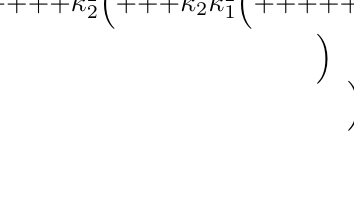
\begin{tikzpicture}[
  every node/.style={inner sep=1pt, circle, draw, fill=white, thin},
  label/.style={draw=none, fill=none, text=black, font=\scriptsize},
  declare function={
    xgap=1;  % Horizontal spacing between diagrams
    ygap=.6;  % Vertical spacing between rows
  },
  baseline=-1cm
  ]
  \pgfmathsetmacro{\outerRadius}{.3}
  \pgfmathsetmacro{\innerRadius}{.1}

  % Pattern {4} - 1 partition
  \drawPartitionAtAngle{(0,0)}{4}{$\kappa_4$}{{{1,2,3,4}}}

  % Pattern {3,1} - 4 partitions
  \drawPartitionAtAngle{(0,-ygap)}{4}{$+\kappa_3\kappa_1\Big($}{{{1,2,3},{4}}}
  \drawPartitionAtAngle{(xgap,-ygap)}{4}{$+$}{{{1,2,4},{3}}}
  \drawPartitionAtAngle{(2*xgap,-ygap)}{4}{$+$}{{{2},{1,3,4}}}
  \drawPartitionAtAngle{(3*xgap,-ygap)}{4}{$+$}{{{1},{2,3,4}}}
  \node[label] at (3.5*xgap,-ygap) {$\Big)$};

  % Pattern {2,2} - 3 partitions
  \drawPartitionAtAngle{(0,-2*ygap)}{4}{$+\kappa_2^2\Big($}{{{1,2},{3,4}}}
  \drawPartitionAtAngle{(xgap,-2*ygap)}{4}{$+$}{{{1,3},{2,4}}}
  \drawPartitionAtAngle{(2*xgap,-2*ygap)}{4}{$+$}{{{1,4},{2,3}}}
  \node[label] at (2.5*xgap,-2*ygap) {$\Big)$};

  % Pattern {2,1,1} - 6 partitions
  \drawPartitionAtAngle{(0,-3*ygap)}{4}{$+\kappa_2\kappa_1^2\Big($}{{{1,2},{3},{4}}}
  \drawPartitionAtAngle{(xgap,-3*ygap)}{4}{$+$}{{{1,3},{2},{4}}}
  \drawPartitionAtAngle{(2*xgap,-3*ygap)}{4}{$+$}{{{1,4},{2},{3}}}
  \drawPartitionAtAngle{(3*xgap,-3*ygap)}{4}{$+$}{{{1},{2,3},{4}}}
  \drawPartitionAtAngle{(4*xgap,-3*ygap)}{4}{$+$}{{{1},{3},{2,4}}}
  \drawPartitionAtAngle{(5*xgap,-3*ygap)}{4}{$+$}{{{1},{2},{3,4}}}
  \node[label] at (5.5*xgap,-3*ygap) {$\Big)$};

  % Pattern {1,1,1,1} - 1 partition
  \drawPartitionAtAngle{(0,-4*ygap)}{4}{$+\kappa_1^4$}{{{1},{2},{3},{4}}}

\end{tikzpicture}
\]

Note in particular, that if the mean, $\kappa_1$, is zero, only four terms survive.
%\(
%\begin{tikzpicture}[
%   baseline=4em,
%  every node/.style={inner sep=1pt, circle, draw, fill=white, thin},
%  label/.style={draw=none, fill=none, text=black, font=\scriptsize},
%  declare function={
%    xgap=1;  % Horizontal spacing between diagrams
%    ygap=.6;  % Vertical spacing between rows
%  },
%  baseline=-1cm
%  ]
%  \pgfmathsetmacro{\outerRadius}{.3}
%  \pgfmathsetmacro{\innerRadius}{.1}
%
%  \drawPartitionAtAngle{(-1.5*xgap,0)}{4}{$\kappa_4$}{{{1,2,3,4}}}
%  \drawPartitionAtAngle{(0,0)}{4}{$+\kappa_2^2\Big($}{{{1,2},{3,4}}}
%  \drawPartitionAtAngle{(xgap,0)}{4}{$+$}{{{1,3},{2,4}}}
%  \drawPartitionAtAngle{(2*xgap,0)}{4}{$+$}{{{1,4},{2,3}}}
%  \node[label] at (2.5*xgap,0) {$\Big)$};
%\end{tikzpicture}
%.
%\)
For $n=5$ there are 52 partitions in total, but only 11 survive if $\kappa_1=0$:
\[
   \begin{tikzpicture}[
     every node/.style={inner sep=1pt, circle, draw, fill=white, thin},
     label/.style={draw=none, fill=none, text=black, font=\scriptsize},
     declare function={
       xgap=1;  % Horizontal spacing between diagrams
       ygap=.6;  % Vertical spacing between rows
     },
     baseline=-1cm
     ]
     \pgfmathsetmacro{\outerRadius}{.3}
     \pgfmathsetmacro{\innerRadius}{.1}
   % Pattern {5} - 1 partition
   \drawPartitionAtAngle{(-1.8*xgap,-ygap)}{5}{$\kappa_5$}{{{1,2,3,4,5}}}
   % Pattern {3,2} - 10 partitions
   \drawPartitionAtAngle{(0,-ygap)}{5}{$+\kappa_3\kappa_2\Big($}{{{1,2,3},{4,5}}}
   \drawPartitionAtAngle{(xgap,-ygap)}{5}{$+$}{{{3,5},{1,2,4}}}
   \drawPartitionAtAngle{(2*xgap,-ygap)}{5}{$+$}{{{1,2,5},{3,4}}}
   \drawPartitionAtAngle{(3*xgap,-ygap)}{5}{$+$}{{{1,3,4},{2,5}}}
   \drawPartitionAtAngle{(4*xgap,-ygap)}{5}{$+$}{{{1,3,5},{2,4}}}
   \drawPartitionAtAngle{(5*xgap,-ygap)}{5}{$+$}{{{1,4,5},{2,3}}}
   \drawPartitionAtAngle{(6*xgap,-ygap)}{5}{$+$}{{{1,5},{2,3,4}}}
   \drawPartitionAtAngle{(7*xgap,-ygap)}{5}{$+$}{{{2,3,5},{1,4}}}
   \drawPartitionAtAngle{(8*xgap,-ygap)}{5}{$+$}{{{1,3},{2,4,5}}}
   \drawPartitionAtAngle{(9*xgap,-ygap)}{5}{$+$}{{{1,2},{3,4,5}}}
   \node[label] at (9.5*xgap,-ygap) {$\Big)$};
   \end{tikzpicture}
\]

If $x$ is Gaussian, all cumulants of order $3$ and higher are zero.
For $n=6$ there are 203 partitions in total, but only 15 terms\footnote{This is why $\E[g^6]=15$ for $g\sim N(0,1)$.} for $E[x^{\otimes 6}]$:
\[
   \begin{tikzpicture}[
     every node/.style={inner sep=1pt, circle, draw, fill=white, thin},
     label/.style={draw=none, fill=none, text=black, font=\scriptsize},
     declare function={
       xgap=1;  % Horizontal spacing between diagrams
       ygap=.8;  % Vertical spacing between rows
     },
     baseline=-1cm
     ]
     \pgfmathsetmacro{\outerRadius}{.3}
     \pgfmathsetmacro{\innerRadius}{.1}
     % Pattern {2,2,2} - 15 partitions
     \drawPartitionAtAngle{(0,0)}{6}{$\kappa_2^3\Big($}{{{1,2},{3,4},{5,6}}}
     \drawPartitionAtAngle{(xgap,0)}{6}{$+$}{{{1,2},{3,5},{4,6}}}
     \drawPartitionAtAngle{(2*xgap,0)}{6}{$+$}{{{1,2},{3,6},{4,5}}}
     \drawPartitionAtAngle{(3*xgap,0)}{6}{$+$}{{{1,3},{2,4},{5,6}}}
     \drawPartitionAtAngle{(4*xgap,0)}{6}{$+$}{{{1,3},{2,5},{4,6}}}
     \drawPartitionAtAngle{(5*xgap,0)}{6}{$+$}{{{1,3},{2,6},{4,5}}}
     \drawPartitionAtAngle{(6*xgap,0)}{6}{$+$}{{{1,4},{2,3},{5,6}}}
     % row 2
     \drawPartitionAtAngle{(1*xgap,-ygap)}{6}{$+$}{{{1,4},{2,5},{3,6}}}
     \drawPartitionAtAngle{(2*xgap,-ygap)}{6}{$+$}{{{1,4},{2,6},{3,5}}}
     \drawPartitionAtAngle{(3*xgap,-ygap)}{6}{$+$}{{{1,5},{2,3},{4,6}}}
     \drawPartitionAtAngle{(4*xgap,-ygap)}{6}{$+$}{{{1,5},{2,4},{3,6}}}
     \drawPartitionAtAngle{(5*xgap,-ygap)}{6}{$+$}{{{1,5},{2,6},{3,4}}}
     \drawPartitionAtAngle{(6*xgap,-ygap)}{6}{$+$}{{{1,6},{2,3},{4,5}}}
     \drawPartitionAtAngle{(7*xgap,-ygap)}{6}{$+$}{{{1,6},{3,5},{2,4}}}
     \drawPartitionAtAngle{(8*xgap,-ygap)}{6}{$+$}{{{1,6},{3,4},{2,5}}}
     \node[label] at (8.5*xgap,-ygap) {$\Big)$};
     \end{tikzpicture}
     .
\]

\subsection{Quartic Forms}





We can use this to compute $\mathrm{Var}[x^T A x]$.
We assume $A$ is symmetric:
\begin{walign}
   \mathrm{Var}[x^T A x]
   &=
   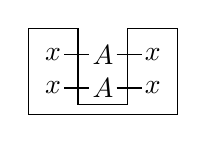
\begin{tikzpicture}[baseline=.5em, inner sep=1pt, x=1.8em, y=1.2em]
      \node (x0) at (0,0) {$x$};
      \node (A0) at (1,0) {$A$};
      \node (x1) at (2,0) {$x$};
      \draw (x0) -- (A0) -- (x1);
      \node (x2) at (0,1) {$x$};
      \node (A1) at (1,1) {$A$};
      \node (x3) at (2,1) {$x$};
      \draw (x2) -- (A1) -- (x3);
      \draw (-.5,-.8) -- (2.5,-.8) -- (2.5,1.8) -- (1.5,1.8) -- (1.5,-.5) -- (.5,-.5) -- (.5,1.8) -- (-.5,1.8) -- (-.5,-.8);
   \end{tikzpicture}
   -
   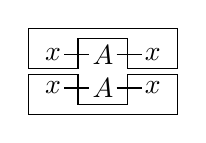
\begin{tikzpicture}[baseline=.5em, inner sep=1pt, x=1.8em, y=1.2em]
      \node (x0) at (0,0) {$x$};
      \node (A0) at (1,0) {$A$};
      \node (x1) at (2,0) {$x$};
      \draw (x0) -- (A0) -- (x1);
      \node (x2) at (0,1) {$x$};
      \node (A1) at (1,1) {$A$};
      \node (x3) at (2,1) {$x$};
      \draw (x2) -- (A1) -- (x3);
      \draw (-.5,-.8) -- (2.5,-.8) -- (2.5,.4) -- (1.5,.4) -- (1.5,-.5) -- (.5,-.5) -- (.5,.4) -- (-.5,.4) -- (-.5,-.8);
      \draw (-.5,1.8) -- (2.5,1.8) -- (2.5,.6) -- (1.5,.6) -- (1.5,1.5) -- (.5,1.5) -- (.5,.6) -- (-.5,.6) -- (-.5,1.8);
   \end{tikzpicture}
   \\&=
   \kappa_4
   \begin{tikzpicture}[baseline=(A0.base), inner sep=0pt, fill=white]
       \node (A1) at (0,0) {$A$};
       \node (bullet) at (.8,0) {$\sbullet$};
       \node[anchor=west] (A2) at (1.4,0) {$A$};
       \draw (A1.east) to[out=45,in=135] (bullet) to[out=45,in=135] (A2.west);
       \draw (A1.east) to[out=-45,in=-135] (bullet) to[out=-45,in=-135] (A2.west);
   \end{tikzpicture}
   +
   4\kappa_3\kappa_1
   \begin{tikzpicture}[baseline=(A0.base), inner sep=1pt]
       \node (A1) at (0,0) {$A$};
       \node (bullet) at (.8,0) {$\sbullet$};
       \node[anchor=west] (A2) at (1.1,0) {$A$};
       \node (bullet2) at (1.8,0) {$\sbullet$};
       \draw (A1.east) to[out=45,in=135] (bullet) -- (A2.west);
       \draw (A1.east) to[out=-45,in=-135] (bullet);
       \draw (A2.east) -- (bullet2);
   \end{tikzpicture}
   \\&\quad+
   2 \kappa_2^2 \hspace{-.5em}\trace{A,A}{2}\hspace{-.5em} + \kappa_2^2 \hspace{-1em}\trace{A}{1}\hspace{-2em}\trace{A}{1}
   \\&\quad+
   4\kappa_2\kappa_1^2
   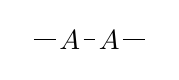
\begin{tikzpicture}[baseline=(A.base), inner sep=1pt]
       \node (bullet) at (0,0) {$\sbullet$};
       \node (A) at (.5,0) {$A$};
       \node (A2) at (1,0) {$A$};
       \node (bullet2) at (1.5,0) {$\sbullet$};
       \draw (bullet.east) -- (A.west);
       \draw (A.east) -- (A2.west);
       \draw (A2.east) -- (bullet2.west);
   \end{tikzpicture}
   +2\kappa_2\kappa_1^2
   \hspace{-1em} \trace{A}{1}\hspace{-1em}
   \vecmatvec{.5em}{\sbullet}{A}{\sbullet}
   \\&\quad+\kappa_1^4 \vecmatvec{.5em}{\sbullet}{A}{\sbullet}
   \vecmatvec{.5em}{\sbullet}{A}{\sbullet}
   \\&\quad-\big(
      \kappa_2 
      \hspace{-1em} \trace{A}{1}\hspace{-1em}
      +
      \kappa_1^2
      \vecmatvec{.5em}{\sbullet}{A}{\sbullet}
   \big)^2
   \\&=
   %%%
   2 \kappa_2^2 \hspace{-.5em}\trace{A,A}{2}\hspace{-.5em}
   +4\kappa_2\kappa_1^2
   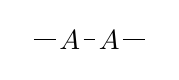
\begin{tikzpicture}[baseline=(A.base), inner sep=1pt]
       \node (bullet) at (0,0) {$\sbullet$};
       \node (A) at (.5,0) {$A$};
       \node (A2) at (1,0) {$A$};
       \node (bullet2) at (1.5,0) {$\sbullet$};
       \draw (bullet.east) -- (A.west);
       \draw (A.east) -- (A2.west);
       \draw (A2.east) -- (bullet2.west);
   \end{tikzpicture}
   \\&\quad+
   4\kappa_3\kappa_1
   \begin{tikzpicture}[baseline=(A0.base), inner sep=1pt]
       \node (A1) at (0,0) {$A$};
       \node (bullet) at (.8,0) {$\sbullet$};
       \node[anchor=west] (A2) at (1.1,0) {$A$};
       \node (bullet2) at (1.8,0) {$\sbullet$};
       \draw (A1.east) to[out=45,in=135] (bullet) -- (A2.west);
       \draw (A1.east) to[out=-45,in=-135] (bullet);
       \draw (A2.east) -- (bullet2);
   \end{tikzpicture}
   +\kappa_4
   \begin{tikzpicture}[baseline=(A0.base), inner sep=0pt, fill=white]
       \node (A1) at (0,0) {$A$};
       \node (bullet) at (.8,0) {$\sbullet$};
       \node[anchor=west] (A2) at (1.4,0) {$A$};
       \draw (A1.east) to[out=45,in=135] (bullet) to[out=45,in=135] (A2.west);
       \draw (A1.east) to[out=-45,in=-135] (bullet) to[out=-45,in=-135] (A2.west);
   \end{tikzpicture}
\end{walign}
The Matrix Cookbook lists this as
\[
   \mathrm{Var}[x^T A x]
   =
   2\mu_2^2\text{Tr}(A^2)
   + 4\mu_2 c^T A^2 c
   + 4\mu_3 c^T Aa
   + (\mu_4 - 3\mu_2^2)a^T a \tag{319}
\]
where $c = \mu_1$ is the mean of $x$,
and $a = \mathrm{diag}(A)$ is the diagonal of $A$,
and $\mu_4 = \kappa_4 + 3\kappa_2^2$ is the fourth central moment.


\section{Weighted Scalar Variable}
Let $y=w^T x$, and let $m=E[y]$, then
\begin{align*}
   \tag{321}
   \E[y] &= m = w^T \mu
   \\
   \tag{322}
   \E[(y\ominus m)^2] &= \vecmatvec{.5em}{w}{M_2}{w}
   \\
   \tag{323}
   \E[(y\ominus m)^3] &=
   \mathbin{\begin{tikzpicture}[baseline=(a0.base), inner sep=1pt]
      \node (a0) {$M_3$};
      \node[above=.3em of a0] (n0) {$w$};
      \node[right=.3em of a0] (n1) {$w$};
      \node[left=.3em of a0] (n3) {$w$};
      \draw (a0.north) -- (n0);
      \draw (a0.east) -- (n1);
      \draw (a0.west) -- (n3);
   \end{tikzpicture}}
   \\
   \tag{324}
   \E[(y\ominus m)^4] &=
   \mathbin{\begin{tikzpicture}[baseline=(a0.base), inner sep=1pt]
      \node (a0) {$M_4$};
      \node[above=.3em of a0] (n0) {$w$};
      \node[right=.3em of a0] (n1) {$w$};
      \node[below=.3em of a0] (n2) {$w$};
      \node[left=.3em of a0] (n3) {$w$};
      \draw (a0.north) -- (n0);
      \draw (a0.east) -- (n1);
      \draw (a0.south) -- (n2);
      \draw (a0.west) -- (n3);
   \end{tikzpicture}}
\end{align*}


For $x\sim N(0,1)$, we have the inequality:
\[
   \E[y^n]^{1/n} \leq \sqrt{2/\pi}\, \|w\|_2.
\]


\section{Gaussian Moments}

For a Gaussian vector $x \sim \mathcal{N}(m,M)$:
- All odd centered moments vanish: $M_3 = 0$, etc.
- Even moments can be computed via Isserlis' theorem.

For instance:
\[
\mathbb{E}[(x \ominus m)^{\otimes 4}]
=
M \otimes M + M \otimes M + \dots
\]
(summing over the different pairings of indices).

\subsection{Gaussian Integration by Parts}
If $X$ is a tensor with Gaussian entries, zero mean, and some covariance,
% General principle for Gaussian expectations.
Stein's lemma gives the following very general equation, for any differentiable function $f$:
\[
   \vcenter{\hbox{
      \import{figures/}{steins.pdf_tex}
   }}
\]
Combined with the tensor chain rule from chapter~\ref{chapter:functions}, this can be a very powerful way to evaluate many hard expectations.



\begin{align*}
E(xx^T) &= \Sigma + mm^T \tag{377} \\
E[x^TAx] &= \text{Tr}(A\Sigma) + m^TAm \tag{378} \\
\text{Var}(x^TAx) &= \text{Tr}[A\Sigma(A + A^T)\Sigma] + \cdots \tag{379} \\
&\quad +m^T(A + A^T)\Sigma(A + A^T)m \\
E[(x - m')^TA(x - m')] &= (m - m')^TA(m - m') + \text{Tr}(A\Sigma) \tag{380}
\end{align*}

If $\Sigma = \sigma^2I$ and $A$ is symmetric, then

\begin{align*}
\text{Var}(x^TAx) = 2\sigma^4\text{Tr}(A^2) + 4\sigma^2m^TA^2m \tag{381}
\end{align*}

Assume $x \sim \mathcal{N}(0, \sigma^2I)$ and $A$ and $B$ to be symmetric, then

\begin{align*}
\text{Cov}(x^TAx, x^TBx) = 2\sigma^4\text{Tr}(AB) \tag{382}
\end{align*}

\subsection{Cubic forms}

Assume $x$ to be a stochastic vector with independent coordinates, mean $m$ and covariance $M$

\begin{align*}
E[xb^Txx^T] &= mb^T(M + mm^T) + (M + mm^T)bm^T \tag{383} \\
&\quad +b^Tm(M - mm^T)
\end{align*}

\subsection{Mean of Quartic Forms}

\begin{align*}
E[xx^Txx^T] &= 2(\Sigma + mm^T)^2 + m^Tm(\Sigma - mm^T) \\
&\quad +\text{Tr}(\Sigma)(\Sigma + mm^T) \\[1em]
E[xx^TAxx^T] &= (\Sigma + mm^T)(A + A^T)(\Sigma + mm^T) \\
&\quad +m^TAm(\Sigma - mm^T) + \text{Tr}[A\Sigma](\Sigma + mm^T) \\[1em]
E[x^Txx^Tx] &= 2\text{Tr}(\Sigma^2) + 4m^T\Sigma m + (\text{Tr}(\Sigma) + m^Tm)^2 \\[1em]
E[x^TAxx^TBx] &= \text{Tr}[A\Sigma(B + B^T)\Sigma] + m^T(A + A^T)\Sigma(B + B^T)m \\
&\quad +(\text{Tr}(A\Sigma) + m^TAm)(\text{Tr}(B\Sigma) + m^TBm)
\end{align*}

\begin{align*}
E[a^Txb^Txc^Txd^Tx] &= (a^T(\Sigma + mm^T)b)(c^T(\Sigma + mm^T)d) \\
&\quad +(a^T(\Sigma + mm^T)c)(b^T(\Sigma + mm^T)d) \\
&\quad +(a^T(\Sigma + mm^T)d)(b^T(\Sigma + mm^T)c) - 2a^Tmb^Tmc^Tmd^Tm
\end{align*}

\begin{align*}
&E[(Ax + a)(Bx + b)^T(Cx + c)(Dx + d)^T] \\
&= [A\Sigma B^T + (Am + a)(Bm + b)^T][C\Sigma D^T + (Cm + c)(Dm + d)^T] \\
&\quad +[A\Sigma C^T + (Am + a)(Cm + c)^T][B\Sigma D^T + (Bm + b)(Dm + d)^T] \\
&\quad +(Bm + b)^T(Cm + c)[A\Sigma D^T - (Am + a)(Dm + d)^T] \\
&\quad +\text{Tr}(B\Sigma C^T)[A\Sigma D^T + (Am + a)(Dm + d)^T]
\end{align*}

\begin{align*}
&E[(Ax + a)^T(Bx + b)(Cx + c)^T(Dx + d)] \\
&= \text{Tr}[A\Sigma(C^TD + D^TC)\Sigma B^T] \\
&\quad +[(Am + a)^TB + (Bm + b)^TA]\Sigma[C^T(Dm + d) + D^T(Cm + c)] \\
&\quad +[\text{Tr}(A\Sigma B^T) + (Am + a)^T(Bm + b)][\text{Tr}(C\Sigma D^T) + (Cm + c)^T(Dm + d)]
\end{align*}

See [7].


\subsection{Mixture of Gaussians}
For a mixture of Gaussians:
\[
   x \sim \sum_k \pi_k \mathcal{N}(m_k, M_k),
\]
the moments are weighted sums:
\[
   E[x] = \sum_k \pi_k m_k, \quad
   \mathrm{Var}[x] = \sum_k \pi_k (M_k + m_k m_k^T) - \left(\sum_k \pi_k m_k\right)\left(\sum_k \pi_k m_k\right)^T.
\]
Higher moments similarly combine via linearity.


\begin{align*}
E[x] &= \sum_k \rho_k m_k \tag{384} \\[1em]
\text{Cov}(x) &= \sum_k\sum_{k'} \rho_k\rho_{k'} (\Sigma_k + m_km_k^T - m_km_{k'}^T) \tag{385}
\end{align*}

\subsection{Derivatives}
Derivatives of moments with respect to $m$ or $M$ can be found by differentiating under the integral sign, and using Stein's lemma for Gaussian cases.

\section{Free Probability for Vectors and Tensors}

Free probability theory provides a non-commutative analogue of classical probability. We'll start with the simplest case—vectors with scalar entries—then progress to matrices and finally to higher-rank tensors.

\subsection{Free Cumulants for Vectors}

For a random vector $x \in \mathbb{R}^n$ with scalar entries, free cumulants are defined analogously to classical cumulants but using only non-crossing partitions.

\subsubsection{R-Transform for Vectors}

The R-transform (free cumulant generating function) is:
\[
   R_x(z) = \sum_{n=1}^{\infty} \kappa_n^{\text{free}} z^{n-1}
\]

This is the free analogue of the classical cumulant generating function $\log \mathrm{E}[e^{tz}] = \sum_{n=1}^{\infty} \frac{\kappa_n}{n!} t^n$.

\subsubsection{Moment-Cumulant Relations}

If each $x_i$ has free cumulants $\kappa_1^{\text{free}}, \kappa_2^{\text{free}}, \kappa_3^{\text{free}}, \kappa_4^{\text{free}} \in \mathbb{R}$, then:
\[
\begin{bmatrix}
   \begin{tikzpicture}[
      baseline=(T.base),
      every node/.style={inner sep=1pt, circle, draw=none, fill=white},
    ]
    \draw (30:.2) node[label] {$x$} -- (30:.5);
    \draw (120:.2) node[label] {$x$} -- (120:.5);
    \draw (210:.2) node[label] {$x$} -- (210:.5);
    \draw (300:.2) node[label] {$x$} -- (300:.5);
   \end{tikzpicture}
\end{bmatrix}_{\text{free}}
=
\begin{tikzpicture}[
  every node/.style={inner sep=1pt, circle, draw, fill=white, thin},
  label/.style={draw=none, fill=none, text=black, font=\scriptsize},
  crossing/.style={draw=red, fill=red!20},
  declare function={
    xgap=1;
    ygap=.6;
  },
  baseline=-1cm
  ]
  
  % Pattern {4} - 1 partition (non-crossing)
  \drawPartitionAtAngle{(0,0)}{4}{$\kappa_4^{\text{free}}$}{{{1,2,3,4}}}

  % Pattern {3,1} - 4 partitions total
  \drawPartitionAtAngle{(0,-ygap)}{4}{$+\kappa_3^{\text{free}}\kappa_1^{\text{free}}\Big($}{{{1,2,3},{4}}}
  \drawPartitionAtAngle[crossing]{(xgap,-ygap)}{4}{$\times$}{{{1,2,4},{3}}}
  \drawPartitionAtAngle[crossing]{(2*xgap,-ygap)}{4}{$\times$}{{{2},{1,3,4}}}
  \drawPartitionAtAngle{(3*xgap,-ygap)}{4}{$+$}{{{1},{2,3,4}}}
  \node[label] at (3.5*xgap,-ygap) {$\Big)$};

  % Pattern {2,2} - 3 partitions total
  \drawPartitionAtAngle{(0,-2*ygap)}{4}{$+(\kappa_2^{\text{free}})^2\Big($}{{{1,2},{3,4}}}
  \drawPartitionAtAngle[crossing]{(xgap,-2*ygap)}{4}{$\times$}{{{1,3},{2,4}}}
  \drawPartitionAtAngle{(2*xgap,-2*ygap)}{4}{$+$}{{{1,4},{2,3}}}
  \node[label] at (2.5*xgap,-2*ygap) {$\Big)$};

  % Pattern {2,1,1} - 6 partitions total
  \drawPartitionAtAngle{(0,-3*ygap)}{4}{$+\kappa_2^{\text{free}}(\kappa_1^{\text{free}})^2\Big($}{{{1,2},{3},{4}}}
  \drawPartitionAtAngle[crossing]{(xgap,-3*ygap)}{4}{$\times$}{{{1,3},{2},{4}}}
  \drawPartitionAtAngle[crossing]{(2*xgap,-3*ygap)}{4}{$\times$}{{{1,4},{2},{3}}}
  \drawPartitionAtAngle[crossing]{(3*xgap,-3*ygap)}{4}{$\times$}{{{1},{2,3},{4}}}
  \drawPartitionAtAngle[crossing]{(4*xgap,-3*ygap)}{4}{$\times$}{{{1},{3},{2,4}}}
  \drawPartitionAtAngle{(5*xgap,-3*ygap)}{4}{$+$}{{{1},{2},{3,4}}}
  \drawPartitionAtAngle{(6*xgap,-3*ygap)}{4}{$+$}{{{1,4},{2},{3}}}
  \node[label] at (6.5*xgap,-3*ygap) {$\Big)$};

  % Pattern {1,1,1,1} - 1 partition (non-crossing)
  \drawPartitionAtAngle{(0,-4*ygap)}{4}{$+(\kappa_1^{\text{free}})^4$}{{{1},{2},{3},{4}}}

  % Legend
  \node[label, red] at (4,-5*ygap) {\small Red = crossing partitions (excluded in free probability)};

\end{tikzpicture}
\]

Compare with classical: 15 partitions $\to$ 9 non-crossing partitions!

\subsection{Free Cumulants for Matrices}

For random matrices, we must consider traces of products. Unlike scalars, matrix products don't commute, adding complexity.
\[
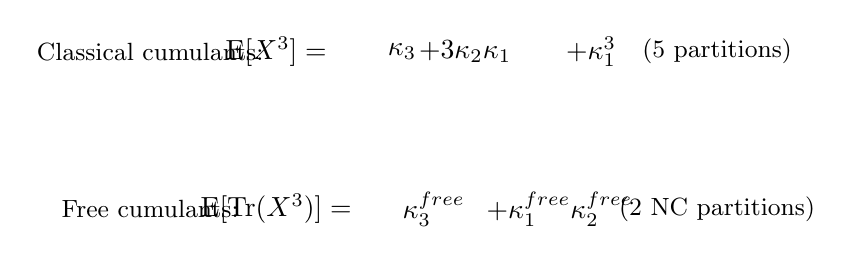
\begin{tikzpicture}[baseline=-.5em, scale=0.8]
   % Classical vs Free
   \node at (-2,1) {\small Classical cumulants:};
   \node at (-2,-1.5) {\small Free cumulants:};
   
   % Classical - all 5 partitions
   \node at (0,1) {$\mathrm{E}[X^3] =$};
   \node at (2,1) {$\kappa_3$};
   \node at (3,1) {$+ 3\kappa_2\kappa_1$};
   \node at (5,1) {$+ \kappa_1^3$};
   \node at (7,1) {\small (5 partitions)};
   
   % Free - only 2 non-crossing
   \node at (0,-1.5) {$\mathrm{E}[\mathrm{Tr}(X^3)] =$};
   \node at (2.5,-1.5) {$\kappa_3^{\text{free}}$};
   \node at (4.5,-1.5) {$+ \kappa_1^{\text{free}}\kappa_2^{\text{free}}$};
   \node at (7,-1.5) {\small (2 NC partitions)};
\end{tikzpicture}
\]

The partition $(1,3),(2)$ is crossing and thus excluded in free probability:
\[
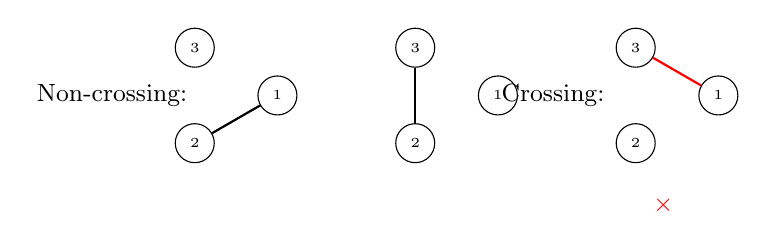
\begin{tikzpicture}[baseline=0, scale=0.7]
   % Non-crossing partitions
   \node at (-2,0) {\small Non-crossing:};
   \foreach \i in {1,2,3} {
      \node[circle, draw] (A\i) at (120-120*\i:1) {\tiny \i};
   }
   \draw[thick] (A1) to (A2);
   \draw[thick] (A3) to (A3);
   
   \begin{scope}[xshift=4cm]
      \foreach \i in {1,2,3} {
         \node[circle, draw] (B\i) at (120-120*\i:1) {\tiny \i};
      }
      \draw[thick] (B1) to (B1);
      \draw[thick] (B2) to (B3);
   \end{scope}
   
   % Crossing partition
   \begin{scope}[xshift=8cm]
      \node at (-2,0) {\small Crossing:};
      \foreach \i in {1,2,3} {
         \node[circle, draw] (C\i) at (120-120*\i:1) {\tiny \i};
      }
      \draw[thick, red] (C1) to (C3);
      \draw[thick] (C2) to (C2);
      \node[red] at (0,-2) {\small $\times$};
   \end{scope}
\end{tikzpicture}
\]

Key insight: For matrices, we have ONE edge to match between elements. For higher-rank tensors, we have MULTIPLE edges (colors) to match.

\subsection{Tensor Free Cumulants}

For rank-$D$ tensors, the free cumulant theory becomes richer due to colored non-crossing partitions.

\subsubsection{Colored Non-Crossing Partitions for Tensors}

For rank-$D$ tensors, each element has $D$ "legs" or indices. A valid pairing must:
\begin{itemize}
\item Be non-crossing when elements are arranged on a circle
\item Match ALL $D$ colors (one per leg) between paired elements
\end{itemize}

This dramatically reduces the number of valid partitions. For rank-3 tensors:
\[
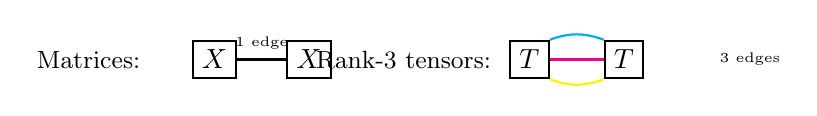
\begin{tikzpicture}[baseline=-.5em, scale=0.8]
   % Matrix case
   \node at (-3,0) {\small Matrices:};
   \node[draw, thick] (M1) at (-1,0) {$X$};
   \node[draw, thick] (M2) at (0.5,0) {$X$};
   \draw[thick] (M1.east) -- (M2.west) node[midway, above] {\tiny 1 edge};
   
   % Tensor case
   \node at (2,0) {\small Rank-3 tensors:};
   \node[draw, thick] (T1) at (4,0) {$T$};
   \node[draw, thick] (T2) at (5.5,0) {$T$};
   % Must connect all 3 colors
   \draw[cyan, thick] (T1.north east) to[bend left=20] (T2.north west);
   \draw[magenta, thick] (T1.east) -- (T2.west);
   \draw[yellow, thick] (T1.south east) to[bend right=20] (T2.south west);
   \node at (7.5,0) {\tiny 3 edges};
\end{tikzpicture}
\]

\subsubsection{Invariant Traces for Tensors}

Unlike matrices, higher-rank tensors have no single canonical trace. Instead, every way of contracting tensors to produce a scalar defines a different invariant:

\begin{center}
\begin{tabular}{|l|l|}
\hline
Matrices ($D=2$) & Tensors ($D>2$) \\
\hline
Unique invariant $\mathrm{Tr}(X_1 \cdots X_n)$ & Family of invariants $\mathrm{Tr}_{\pi}(T_1,\ldots,T_n)$ \\
& indexed by colored permutations $\pi \in \mathfrak{S}_{Dn}$ \\
\hline
\end{tabular}
\end{center}

\textbf{Definition of $\mathrm{Tr}_{\pi}$:} Given tensors $T_1,\ldots,T_n$ each with $D$ legs (colored 1 through $D$), a colored permutation $\pi = (\pi^{(1)},\ldots,\pi^{(D)}) \in \mathfrak{S}_n^D$ specifies which legs connect:

\[
\mathrm{Tr}_{\pi}(T_1,\ldots,T_n) = 
\begin{tikzpicture}[baseline=0, scale=0.8]
   % Example for n=3, D=3
   \node at (-2,0) {\small Example:};
   % Three tensors
   \node[draw, thick] (T1) at (90:1.2) {$T_1$};
   \node[draw, thick] (T2) at (210:1.2) {$T_2$};
   \node[draw, thick] (T3) at (330:1.2) {$T_3$};
   
   % Permutation pi^(1) for cyan: (1 2 3)
   \draw[cyan, thick] (T1) to[bend right=30] node[midway, left] {\tiny $\pi^{(1)}$} (T2);
   \draw[cyan, thick] (T2) to[bend right=30] (T3);
   \draw[cyan, thick] (T3) to[bend right=30] (T1);
   
   % Permutation pi^(2) for magenta: (1 3 2)
   \draw[magenta, thick] (T1) to[bend left=20] node[midway, right] {\tiny $\pi^{(2)}$} (T3);
   \draw[magenta, thick] (T3) to[bend left=20] (T2);
   \draw[magenta, thick] (T2) to[bend left=20] (T1);
   
   % Permutation pi^(3) for yellow: (1)(2)(3)
   \draw[yellow, thick] (T1) to[out=60,in=120,looseness=8] (T1);
   \draw[yellow, thick] (T2) to[out=180,in=240,looseness=8] (T2);
   \draw[yellow, thick] (T3) to[out=300,in=360,looseness=8] (T3);
\end{tikzpicture}
\]

For matrices ($D=2$), only the cyclic permutation gives a non-zero trace, recovering the usual $\mathrm{Tr}(X_1 X_2 \cdots X_n)$.

\textbf{Normalization:} To obtain finite limits as $N \to \infty$, we normalize by $N^{-(D-1)n}$:
\[
   \frac{1}{N^{(D-1)n}} \mathrm{Tr}_{\pi}(T_1,\ldots,T_n) \xrightarrow{N \to \infty} \text{finite}
\]

\subsubsection{Moment-Cumulant Formula}

The tensor moment-cumulant relation involves ALL invariant traces:
\[
   \boxed{\left( \mathrm{E}[\mathrm{Tr}_{\pi}(T_{i_1},\ldots,T_{i_n})] \right)_{\pi \in \mathrm{NC}_D(n)} = \sum_{\sigma \in \mathrm{NC}_D(n)} \kappa_{\sigma}^{(\mathrm{t})} \cdot (\text{pattern matching})}
\]

The moments form a vector indexed by colored non-crossing permutations, and tensor freeness acts on this entire family.

Example for $n=2$: The second moment decomposes as
\[
\begin{tikzpicture}[baseline=-.5em, scale=0.8]
   % Moment
   \node at (-1,0) {$\mathrm{E}[\mathrm{Tr}(T_1 T_2)]$};
   \node at (1,0) {$=$};
   
   % First term: partition (1,2)
   \node at (2.5,0) {$\kappa_2^{(\mathrm{t})}$};
   \node[circle, draw, inner sep=1pt] (A1) at (3.5,0.3) {\tiny 1};
   \node[circle, draw, inner sep=1pt] (A2) at (3.5,-0.3) {\tiny 2};
   \draw[thick] (A1) -- (A2);
   \node at (4.2,0) {$\delta_{i_1,i_2}$};
   
   \node at (5.5,0) {$+$};
   
   % Second term: partition (1),(2)
   \node at (6.5,0) {$(\kappa_1^{(\mathrm{t})})^2$};
   \node[circle, draw, inner sep=1pt] (B1) at (7.5,0.3) {\tiny 1};
   \node[circle, draw, inner sep=1pt] (B2) at (7.5,-0.3) {\tiny 2};
\end{tikzpicture}
\]

For Gaussian tensors, $\kappa_1^{(\mathrm{t})} = 0$ and $\kappa_n^{(\mathrm{t})} = 0$ for $n > 2$, so:
\[
   \mathrm{E}[\mathrm{Tr}(T_1 T_2)] = \kappa_2^{(\mathrm{t})} \delta_{i_1,i_2} = \delta_{i_1,i_2}
\]

\subsection{Tensor Wick Theorem}

For Gaussian tensors, a fundamental result analogous to Wick's theorem holds:

Tensor Wick Factorization:
Let $(T_i)_{i \in I}$ be i.i.d. standard Gaussian $D$-leg tensors of size $N$. As $N \to \infty$:
\[
   \mathrm{E}[T_{i_1} \cdots T_{i_{2k}}] = \sum_{\pi \in \mathrm{NC}_D(2k)} \prod_{(j,j') \in \pi} \delta_{i_j, i_{j'}} + O(N^{-1})
\]

This shows that Gaussian tensors are asymptotically tensor-free, with all cumulants beyond the second vanishing.

For four rank-3 tensors, the valid colored non-crossing pairings are severely restricted:
\[
\begin{tikzpicture}[baseline=-.5em, scale=0.7]
   % First row - tensors arranged in circle
   \node at (-2,2) {\small Tensors arranged on circle:};
   \foreach \i in {1,2,3,4} {
      \node[draw, thick] (T\i) at (90-90*\i:1.5) {$T_{\i}$};
   }
   
   % Second row - valid pairing (1,2)(3,4)
   \begin{scope}[yshift=-4cm]
      \node at (-2,0) {\small $(1,2)(3,4)$ valid:};
      \foreach \i in {1,2,3,4} {
         \node[draw, thick] (S\i) at (90-90*\i:1.5) {$T_{\i}$};
      }
      % Connect 1-2 with all three colors
      \draw[cyan, thick] (S1) to[bend right=20] (S2);
      \draw[magenta, thick] (S1) to (S2);
      \draw[yellow, thick] (S1) to[bend left=20] (S2);
      % Connect 3-4 with all three colors
      \draw[cyan, thick] (S3) to[bend right=20] (S4);
      \draw[magenta, thick] (S3) to (S4);
      \draw[yellow, thick] (S3) to[bend left=20] (S4);
   \end{scope}
   
   % Third row - invalid pairing (1,3)(2,4)
   \begin{scope}[yshift=-8cm]
      \node at (-2,0) {\small $(1,3)(2,4)$ invalid:};
      \foreach \i in {1,2,3,4} {
         \node[draw, thick] (R\i) at (90-90*\i:1.5) {$T_{\i}$};
      }
      % Try to connect 1-3
      \draw[cyan, thick] (R1) to[bend left=45] (R3);
      % This forces 2-4 to cross!
      \draw[red, thick, dashed] (R2) to (R4) node[midway, above] {\tiny crosses!};
   \end{scope}
   
   \node at (5,-4) {\small Only $(1,2)(3,4)$ and $(1,4)(2,3)$ are non-crossing};
\end{tikzpicture}
\]

\subsection{Additivity Under Tensor Freeness}

If two tensor algebras $\mathcal{A}_1$ and $\mathcal{A}_2$ are tensor-free, then for $A \in \mathcal{A}_1$ and $B \in \mathcal{A}_2$:
\[
   \kappa_n^{(\mathrm{t})}(A + B) = \kappa_n^{(\mathrm{t})}(A) + \kappa_n^{(\mathrm{t})}(B)
\]

This generalizes the additivity of classical cumulants for independent variables.

Graphically, for the second cumulant (covariance):
\[
\begin{tikzpicture}[baseline=-.5em, scale=0.8]
   % Left side
   \node at (-1,0) {$\kappa_2^{(\mathrm{t})}\Big($};
   \node[draw, thick] (A) at (0,.5) {$A$};
   \node at (.5,0) {$+$};
   \node[draw, thick] (B) at (1,-.5) {$B$};
   \node at (1.5,0) {$\Big)$};
   
   % Equals
   \node at (2.5,0) {$=$};
   
   % Right side
   \node at (3.5,0) {$\kappa_2^{(\mathrm{t})}$};
   \node[draw, thick] (A2) at (4.5,0) {$A$};
   \draw[thick] (A2) -- ++(-.5,0);
   \draw[thick] (A2) -- ++(.5,0);
   
   \node at (5.5,0) {$+$};
   
   \node at (6.5,0) {$\kappa_2^{(\mathrm{t})}$};
   \node[draw, thick] (B2) at (7.5,0) {$B$};
   \draw[thick] (B2) -- ++(-.5,0);
   \draw[thick] (B2) -- ++(.5,0);
\end{tikzpicture}
\]

\subsubsection{Vanishing Mixed Cumulants}

For matrices, if $A$ and $B$ are free and one has zero trace, then $\kappa_n^{\text{free}}(AB\cdots) = 0$ for alternating products. For tensors, the analogous property depends on the contraction pattern.

\textbf{Definition:} A tensor $T$ has \emph{zero first cumulant} if $\kappa_1^{(\mathrm{t})}(T) = 0$, which means $\mathrm{E}[\mathrm{Tr}_{\pi}(T)] = 0$ for ALL colored permutations $\pi \in \mathfrak{S}_D$.

\textbf{Definition:} An \emph{alternating contraction pattern} is a way of connecting tensors in a sequence $A_1, B_1, A_2, B_2, \ldots$ where:
\begin{itemize}
\item Tensors appear in alternating order (A, B, A, B, ...)
\item Each tensor's legs are contracted with neighbors (no tensor left isolated)
\item The contraction respects the tensor structure
\end{itemize}

\textbf{Theorem:} If $A$ and $B$ are tensor-free and $\kappa_1^{(\mathrm{t})}(A) = 0$, then any alternating contraction has vanishing cumulants:
\[
   \kappa_n^{(\mathrm{t})}(A \otimes_C B \otimes_C A \otimes_C \cdots) = 0 \quad \text{for } n \geq 2
\]

Examples of alternating contractions for rank-3 tensors:
\[
\begin{tikzpicture}[baseline=0, scale=0.7]
   % Example 1: Linear chain
   \node at (-2,1) {\small Linear chain:};
   \node[draw, thick] (A1) at (0,1) {$A$};
   \node[draw, thick] (B1) at (1.5,1) {$B$};
   \node[draw, thick] (A2) at (3,1) {$A$};
   \node[draw, thick] (B2) at (4.5,1) {$B$};
   % Connect with one color
   \draw[cyan, thick] (A1) -- (B1) -- (A2) -- (B2);
   % Other legs free
   \draw[magenta, thick] (A1) -- ++(0,.3);
   \draw[yellow, thick] (A1) -- ++(0,-.3);
   \draw[magenta, thick] (B1) -- ++(0,.3);
   \draw[yellow, thick] (B1) -- ++(0,-.3);
   
   % Example 2: Cyclic
   \node at (-2,-1) {\small Cyclic:};
   \node[draw, thick] (A3) at (0,-1) {$A$};
   \node[draw, thick] (B3) at (1.5,-1) {$B$};
   \node[draw, thick] (A4) at (3,-1) {$A$};
   \node[draw, thick] (B4) at (4.5,-1) {$B$};
   % Connect in a more complex pattern
   \draw[cyan, thick] (A3) -- (B3);
   \draw[magenta, thick] (B3) -- (A4);
   \draw[yellow, thick] (A4) -- (B4);
   \draw[cyan, thick] (B4) to[bend right=30] (A3);
   
   % Example 3: Tree-like
   \node at (-2,-3) {\small Tree:};
   \node[draw, thick] (A5) at (1.5,-3) {$A$};
   \node[draw, thick] (B5) at (0,-3.7) {$B$};
   \node[draw, thick] (B6) at (3,-3.7) {$B$};
   \draw[cyan, thick] (A5) -- (B5);
   \draw[magenta, thick] (A5) -- (B6);
   \draw[yellow, thick] (B5) -- ++(-.5,0);
   \draw[yellow, thick] (B6) -- ++(.5,0);
\end{tikzpicture}
\]

If $\kappa_1^{(\mathrm{t})}(A) = 0$, all these contractions yield $\kappa_n^{(\mathrm{t})} = 0$.

This holds because any non-crossing partition must include a singleton block containing $A$, but $\kappa_1^{(\mathrm{t})}(A) = 0$.

The key difference from matrices: for tensors, we must specify the contraction pattern, as different contractions can yield different results even for the same tensors.

\subsection{Spectrum of Tensor Wishart Matrices}

Consider a rank-3 tensor $T \in \mathbb{C}^{N \times N \times N}$ with i.i.d. Gaussian entries $\mathcal{N}_{\mathbb{C}}(0, N^{-3})$. The Wishart-type matrix $W = TT^{\dagger}$ (contracting one index) has limiting spectral distribution:

\[
\begin{tikzpicture}[baseline=-.5em, scale=0.8]
   % Tensor contraction
   \node[draw, thick] (T1) at (0,0) {$T$};
   \node[draw, thick] (T2) at (2,0) {$T^{\dagger}$};
   \draw[cyan, thick] (T1) -- ++(0,.5);
   \draw[magenta, thick] (T1) to[out=-150,in=-30] (T2);
   \draw[yellow, thick] (T1) -- ++(0,-.5);
   \draw[cyan, thick] (T2) -- ++(0,.5);
   \draw[magenta, thick] (T2) -- ++(0,-.5);
   \draw[yellow, thick] (T2) -- ++(.5,0);
   \node at (3.5,0) {$\xrightarrow{N \to \infty}$};
   \node at (6,0) {$\mathrm{MP}(1) \boxtimes \mathrm{MP}(1) = \mathrm{MP}(1/2)$};
\end{tikzpicture}
\]

where $\boxtimes$ denotes free multiplicative convolution and $\mathrm{MP}(c)$ is the Marchenko-Pastur distribution.

\subsection{Tensor Networks and Free Probability}

Free probability provides powerful tools for analyzing tensor network states, which arise naturally in quantum many-body physics and machine learning.

\subsubsection{Graph Amalgamation}

For a tensor network on a graph $G = (V, E)$ with random Gaussian tensors at each vertex, the boundary density matrix factorizes according to the graph's structure:

Graph Amalgamation:
Let $\rho_b$ be the boundary density matrix of a random tensor network. Then:
\[
   \rho_b = \underset{\gamma \in \mathcal{C}_{\min}}{*_{\mathcal{B}}} \rho_{\gamma}
\]
where $*_{\mathcal{B}}$ denotes free multiplicative convolution with amalgamation over the boundary algebra, and $\mathcal{C}_{\min}$ are the minimal cuts of $G$.

For example, a simple two-vertex network:
\[
\begin{tikzpicture}[baseline=0, scale=0.8]
   % Two tensors
   \node[draw, thick, circle] (T1) at (0,0) {$T_1$};
   \node[draw, thick, circle] (T2) at (3,0) {$T_2$};
   % Internal edge
   \draw[thick] (T1) -- (T2) node[midway, above] {$e$};
   % Boundary edges
   \draw[thick] (T1) -- ++(-1,.5) node[left] {$\partial_1$};
   \draw[thick] (T1) -- ++(-1,-.5) node[left] {$\partial_2$};
   \draw[thick] (T2) -- ++(1,.5) node[right] {$\partial_3$};
   \draw[thick] (T2) -- ++(1,-.5) node[right] {$\partial_4$};
   % Minimal cut
   \draw[dashed, red, thick] (1.5,-1) -- (1.5,1) node[above] {cut};
\end{tikzpicture}
\]

\subsubsection{Entanglement and Max-Flow}

The Rényi entropy of tensor network states connects to max-flow problems on the network graph:

\[
   S_q(\rho_b) = \frac{1}{1-q} \log \left[ \max_f \prod_{e \in E} w_e^{f(e)} \right] + o(1)
\]

where $f$ ranges over integer flows and $w_e$ are edge weights. For maximally entangled links ($w_e = 1$), this recovers the Ryu-Takayanagi formula from holography.

\subsection{Examples with Higher-Order Tensors}

\subsubsection{Star Network}
Consider a star graph with one central vertex of degree $D = 4$:
\[
\begin{tikzpicture}[baseline=0, scale=0.8]
   \node[circle, draw, thick] (C) at (0,0) {$T$};
   \foreach \i in {1,2,3,4} {
      \node (B\i) at (90*\i:1.5) {$\partial_\i$};
      \draw[thick] (C) -- (B\i);
   }
\end{tikzpicture}
\]

The boundary density matrix is $\rho_b = W_1 W_2 W_3 W_4$ with independent Wishart factors. By tensor freeness:
\[
   \mu_{\rho} = \mathrm{MP}(1)^{\boxtimes 4}, \quad R_{\rho}(w) = \frac{4w}{1-w}
\]

The von Neumann entropy per site equals $\log 4 - 3/4$.

The free product decomposition:
\[
\begin{tikzpicture}[baseline=0, scale=0.7]
   % Central tensor with 4 Wishart factors
   \node[circle, draw, thick] (C) at (0,0) {$T$};
   \foreach \i in {1,2,3,4} {
      \node[draw, thick] (W\i) at (90*\i:2) {$W_{\i}$};
      \draw[thick] (C) -- (W\i);
   }
   % Free product symbol
   \node at (3,0) {$=$};
   \node at (4.5,0) {$W_1 \boxtimes W_2 \boxtimes W_3 \boxtimes W_4$};
\end{tikzpicture}
\]

\subsubsection{Ladder Networks}
For a $2 \times L$ ladder with periodic vertical boundary:
\[
\begin{tikzpicture}[baseline=0, scale=0.6]
   \foreach \i in {0,1,2} {
      \node[circle, draw] (T\i) at (1.5*\i,0) {};
      \node[circle, draw] (B\i) at (1.5*\i,-1.5) {};
      \draw (T\i) -- (B\i);
   }
   \node at (4.5,0) {$\cdots$};
   \node at (4.5,-1.5) {$\cdots$};
   \foreach \i in {0,1} {
      \draw (T\i) -- (T\the\numexpr\i+1);
      \draw (B\i) -- (B\the\numexpr\i+1);
   }
\end{tikzpicture}
\]

The entanglement entropy scales as $S_2 = \lceil L/2 \rceil \log N + O(1)$, exhibiting area law scaling.

The max-flow through the network:
\[
\begin{tikzpicture}[baseline=0, scale=0.5]
   % Flow network representation
   \foreach \i in {0,1,2} {
      \foreach \j in {0,1} {
         \node[circle, draw, inner sep=1pt] (T\i\j) at (2*\i,1.5*\j) {};
      }
   }
   % Horizontal edges with flow
   \foreach \i in {0,1} {
      \draw[thick, ->] (T\i0) -- (T\the\numexpr\i+1\relax0) node[midway, above, font=\tiny] {$f_1$};
      \draw[thick, ->] (T\i1) -- (T\the\numexpr\i+1\relax1) node[midway, above, font=\tiny] {$f_2$};
   }
   % Vertical edges
   \foreach \i in {0,1,2} {
      \draw[thick] (T\i0) -- (T\i1);
   }
   % Source and sink
   \node at (-1,0.75) {$s$};
   \node at (5,0.75) {$t$};
   \draw[thick, ->] (-0.5,0.75) -- (T00);
   \draw[thick, ->] (-0.5,0.75) -- (T01);
   \draw[thick, ->] (T20) -- (4.5,0.75);
   \draw[thick, ->] (T21) -- (4.5,0.75);
   % Max flow
   \node at (6,0.75) {$f_{\max} = 2$};
\end{tikzpicture}
\]

\subsection{D-ary Catalan Numbers}

The colored Möbius function for $\mathrm{NC}_D(n)$ involves $D$-ary Catalan numbers:
\[
   \mu_{\mathrm{col}}(0_n, 1_n) = (-1)^{n-1} C_{n-1}^{(D)}
\]

where $C_n^{(D)} = \frac{1}{(D-1)n+1}\binom{Dn}{n}$ are the Fuss-Catalan numbers.

The growth of $D$-ary Catalan numbers:
\[
\begin{tikzpicture}[baseline=0, scale=0.6]
   % Table of values
   \node at (0,2) {$n$};
   \node at (1.5,2) {$C_n^{(2)}$};
   \node at (3,2) {$C_n^{(3)}$};
   \node at (4.5,2) {$C_n^{(4)}$};
   \draw[thick] (-0.5,1.7) -- (5,1.7);
   \foreach \n/\c2/\c3/\c4 in {0/1/1/1, 1/1/1/1, 2/2/3/5, 3/5/12/35, 4/14/55/285} {
      \node at (0,1.3-0.4*\n) {$\n$};
      \node at (1.5,1.3-0.4*\n) {$\c2$};
      \node at (3,1.3-0.4*\n) {$\c3$};
      \node at (4.5,1.3-0.4*\n) {$\c4$};
   }
\end{tikzpicture}
\]

For $D = 2$ (matrices), we recover the standard Catalan numbers. For $D = 3$ (rank-3 tensors):
\[
   C_0^{(3)} = 1, \quad C_1^{(3)} = 1, \quad C_2^{(3)} = 3, \quad C_3^{(3)} = 12, \quad C_4^{(3)} = 55, \ldots
\]

\subsection{Melonic Diagrams}

Melonic diagrams are the leading-order Feynman diagrams in the $1/N$ expansion of tensor models. They are named after their melon-like shape and have a special topological structure.

\subsubsection{Definition and Structure}

For rank-$D$ tensors, a melonic diagram is one that can be drawn on a 2-sphere where:
\begin{itemize}
\item Each face is colored by one of $D$ colors
\item The diagram has a tree-like structure of "melons"
\item No color appears twice around any vertex
\end{itemize}

The basic melon (2-point function) for rank-3 tensors:
\[
\begin{tikzpicture}[baseline=0, scale=0.8]
   % Basic melon
   \node at (-2,0) {Basic melon:};
   \node[circle, draw, thick] (L) at (0,0) {$T$};
   \node[circle, draw, thick] (R) at (2,0) {$\bar{T}$};
   % Three colored edges forming the melon
   \draw[cyan, thick] (L) to[bend left=40] node[above] {\tiny cyan} (R);
   \draw[magenta, thick] (L) to node[below] {\tiny magenta} (R);
   \draw[yellow, thick] (L) to[bend right=40] node[below] {\tiny yellow} (R);
\end{tikzpicture}
\]

\subsubsection{Higher-Order Melonic Diagrams}

The 4-point melonic diagram (order $N^{-1}$):
\[
\begin{tikzpicture}[baseline=0, scale=0.7]
   % 4-point melon
   \node at (-3,0) {4-point:};
   \node[circle, draw, fill=white] (T1) at (0,1) {$T$};
   \node[circle, draw, fill=white] (T2) at (2,1) {$\bar{T}$};
   \node[circle, draw, fill=white] (T3) at (2,-1) {$T$};
   \node[circle, draw, fill=white] (T4) at (0,-1) {$\bar{T}$};
   
   % Internal face (white)
   \draw[thick] (T1) -- (T2) -- (T3) -- (T4) -- (T1);
   
   % External colored faces
   \draw[cyan, thick] (T1) to[bend left=45] (T2);
   \draw[magenta, thick] (T2) to[bend left=45] (T3);
   \draw[yellow, thick] (T3) to[bend left=45] (T4);
   \draw[cyan, thick] (T4) to[bend left=45] (T1);
\end{tikzpicture}
\quad
\begin{tikzpicture}[baseline=0, scale=0.7]
   % Tree structure
   \node at (-2,0) {Tree of melons:};
   \node[circle, draw, fill=white] (C) at (0,0) {};
   \foreach \i in {0,120,240} {
      \node[circle, draw, fill=white] (T\i) at (\i:1.5) {};
      \node[circle, draw, fill=white] (S\i) at (\i:2.5) {};
   }
   % Connect center to first layer
   \foreach \i in {0,120,240} {
      \draw[thick] (C) -- (T\i);
   }
   % Melons on outer layer
   \draw[cyan, thick] (T0) to[bend left=30] (S0);
   \draw[magenta, thick] (T0) to[bend right=30] (S0);
   \draw[cyan, thick] (T120) to[bend left=30] (S120);
   \draw[yellow, thick] (T120) to[bend right=30] (S120);
   \draw[magenta, thick] (T240) to[bend left=30] (S240);
   \draw[yellow, thick] (T240) to[bend right=30] (S240);
   % Connect melons
   \draw[yellow, thick, bend left=20] (T0) to (T120);
   \draw[magenta, thick, bend left=20] (T120) to (T240);
   \draw[cyan, thick, bend left=20] (T240) to (T0);
\end{tikzpicture}
\]

\subsubsection{Counting Melonic Diagrams}

The number of melonic diagrams grows much slower than general diagrams:

Melonic Dominance:
At order $n$ in the $1/N$ expansion:
\begin{itemize}
\item General diagrams: $\sim (D!)^n n!$ 
\item Melonic diagrams: $\sim D^n \cdot C_{n-1}$ (Catalan numbers)
\end{itemize}

For rank-3 tensors at order 3:
\[
\begin{tikzpicture}[baseline=0, scale=0.6]
   % First melonic diagram
   \begin{scope}[xshift=0cm]
      \node at (0,1.5) {\small Type 1};
      \foreach \i in {0,1,2,3} {
         \node[circle, draw, fill=white, inner sep=1pt] (T\i) at (90*\i:1) {};
      }
      \draw[thick] (T0) -- (T1) -- (T2) -- (T3) -- (T0);
      \draw[cyan, thick, bend left=45] (T0) to (T1);
      \draw[magenta, thick, bend left=45] (T1) to (T2);
      \draw[yellow, thick, bend left=45] (T2) to (T3);
      \draw[cyan, thick, bend left=45] (T3) to (T0);
   \end{scope}
   
   % Second melonic diagram
   \begin{scope}[xshift=5cm]
      \node at (0,1.5) {\small Type 2};
      \node[circle, draw, fill=white, inner sep=1pt] (C) at (0,0) {};
      \foreach \i in {0,120,240} {
         \node[circle, draw, fill=white, inner sep=1pt] (T\i) at (\i:0.8) {};
         \node[circle, draw, fill=white, inner sep=1pt] (S\i) at (\i:1.6) {};
      }
      \foreach \i in {0,120,240} {
         \draw[thick] (C) -- (T\i) -- (S\i);
      }
      \draw[cyan, thick, bend left=30] (T0) to (T120);
      \draw[magenta, thick, bend left=30] (T120) to (T240);
      \draw[yellow, thick, bend left=30] (T240) to (T0);
   \end{scope}
   
   % Third melonic diagram  
   \begin{scope}[xshift=10cm]
      \node at (0,1.5) {\small Type 3};
      \node[circle, draw, fill=white, inner sep=1pt] (L) at (-1,0) {};
      \node[circle, draw, fill=white, inner sep=1pt] (C) at (0,0) {};
      \node[circle, draw, fill=white, inner sep=1pt] (R) at (1,0) {};
      \node[circle, draw, fill=white, inner sep=1pt] (T) at (0,1) {};
      \draw[thick] (L) -- (C) -- (R);
      \draw[thick] (C) -- (T);
      \draw[cyan, thick, bend left=30] (L) to (T);
      \draw[magenta, thick, bend right=30] (L) to (T);
      \draw[yellow, thick, bend left=30] (R) to (T);
      \draw[cyan, thick, bend right=30] (R) to (T);
   \end{scope}
\end{tikzpicture}
\]

\subsubsection{Melonic Universality}

In the large-$N$ limit, tensor models are dominated by melonic diagrams, leading to:
\begin{itemize}
\item Spectral dimension $d_s = 2$ (like branched polymers)
\item Critical exponents independent of $D$ for $D \geq 3$
\item Connection to the Sachdev-Ye-Kitaev (SYK) model in physics
\end{itemize}

This universality is why melonic diagrams are central to understanding tensor models and their continuum limits.

\section{Exercises}
\begin{exercise}
   \begin{align*}
   \mathrm{E}[(A\mathbf{x} + a)(A\mathbf{x} + a)^T (A\mathbf{x} + a)] = 
   \mathrm{Adiag}(A^T A) v_3 \\
   + [2 AMA^T + (A\mathbf{x} + a)(A\mathbf{x} + a)^T] (Am + a) \\
   + \mathrm{Tr}(AMA^T)(Am + a)
   \end{align*}

   \begin{align*}
   \mathrm{E}[(A\mathbf{x} + a) b^T (C\mathbf{x} + c)(D\mathbf{x} + d)^T] = 
   (A\mathbf{x} + a) b^T (CMD^T + (Cm + c)(Dm + d)^T) \\
   + (AMC^T + (Am + a)(Cm + c)^T) b(Dm + d)^T \\
   + b^T (Cm + c)(AMD^T - (Am + a)(Dm + d)^T)
   \end{align*}
\end{exercise}
\begin{exercise}
   Find more identities in the \href{http://www.ee.ic.ac.uk/hp/staff/dmb/matrix/expect.html}{Matrix Reference Manual} and try to prove them.
   Also try to verify your derivations using tensorgrad.
\end{exercise}
\begin{exercise}
   For rank-3 tensors $T_1, T_2, T_3$ with colored legs (cyan, magenta, yellow), draw all valid 3-colored non-crossing partitions of $\{1,2,3\}$. 
   How many are there compared to the total number of set partitions?
\end{exercise}
\begin{exercise}
   Consider a rank-4 Gaussian tensor $T \in \mathbb{R}^{N \times N \times N \times N}$. 
   Compute $\mathrm{E}[\mathrm{Tr}_{12}(T) \mathrm{Tr}_{34}(T)]$ where $\mathrm{Tr}_{ij}$ denotes contraction of indices $i$ and $j$.
   Use the tensor Wick theorem and draw the corresponding colored diagrams.
\end{exercise}
\begin{exercise}
   For a tensor network on a binary tree of depth $d$, show that the boundary entanglement entropy scales as $S \sim d \log N$.
   Use the graph amalgamation theorem and identify the minimal cuts.
\end{exercise}
\begin{exercise}
   Verify that for rank-$D$ tensors, the number of melonic diagrams at order $n$ grows as $D^n n!$.
   Draw all melonic diagrams for $D=3, n=3$.
\end{exercise}
\begin{exercise}
   Show that the $D$-ary Catalan numbers satisfy the recursion:
   \[
      C_n^{(D)} = \sum_{k=0}^{n-1} C_k^{(D)} C_{n-1-k}^{(D-1)}
   \]
   What does this imply about the structure of colored non-crossing partitions?
\end{exercise}
\begin{exercise}
   For two tensor-free rank-3 tensors $A$ and $B$, compute the third tensor cumulant $\kappa_3^{(\mathrm{t})}(A+B)$.
   Verify the additivity property using colored partition diagrams.
\end{exercise}
